\subsubsection{Attribution Scores}

\begin{figure}[t]
 	\centering
 	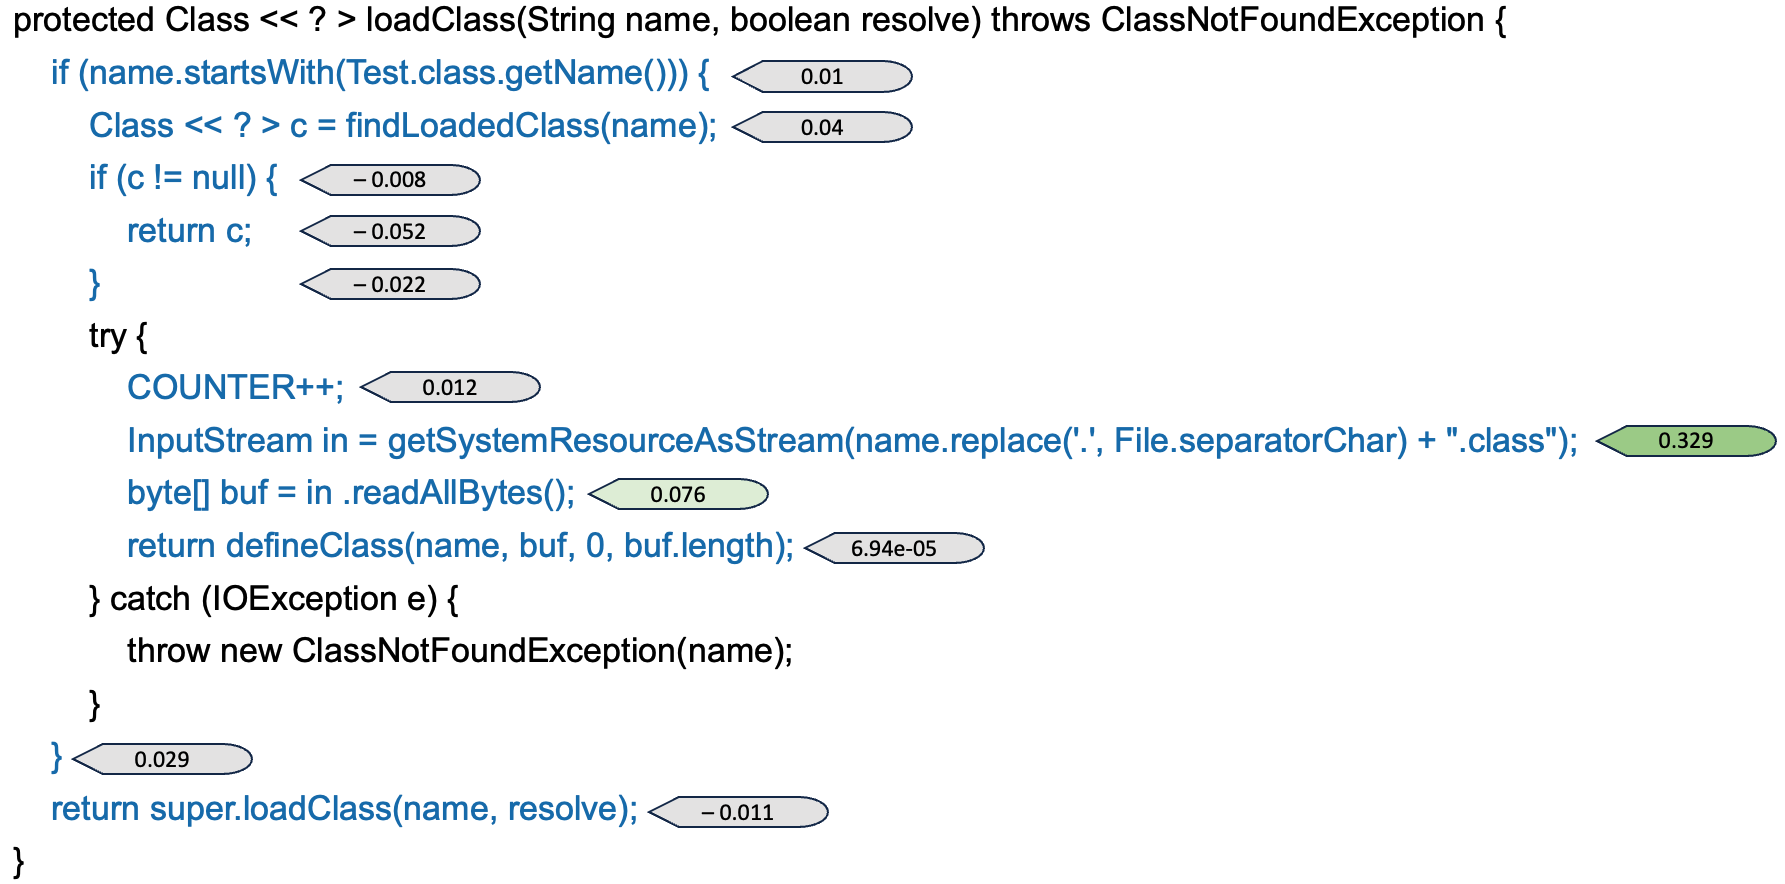
\includegraphics[width=3.4in]{rq1-case-study.png}
        \vspace{-20pt}
 	\caption{{\xblock} Puts Attention on the Right Tokens}
 	\label{fig:rq1-case}	
\end{figure}

%\noindent {\bf Attribution Scores.}

To illustrate how {\xblock} makes the prediction, in
Figure~\ref{fig:rq1-case}, we shows a code snippet that catches an
\code{IOException} thrown by the \code{readAllBytes} API call on an
\code{InputStream} object.
%
We first get the {\em attribution scores} for the input (sub)tokens
via Transformer Interpret~\cite{transformers-interpret}. A higher
attribution score of a token means that the token has more
contribution to the model's prediction. In Figure~\ref{fig:rq1-case},
we show the attribution score for each statement, which is calculated
by averaging the attribution scores of all the sub-tokens in the
statement.
%
%CodeBERT produces as a by-product an {\em attribution score} for each
%code sub-token in the input. The higher the score of a token the
%higher attention that the model pays to that token, contributing to
%the prediction result. In Figure~\ref{fig:rq1-case}, for each
%statement, we show the statement attribution score, which is
%calculated by averaging the attribution scores of all the sub-tokens
%in the statement.
%The number after each statement is the statement attribution score,
%which is calculated by averaging the attribution scores of all the
%sub-tokens in the statement.
%
A positive attribution score means that the statement contributes
positively to the model's predicted class, while a negative score
means the statement contributes negatively to the predicted class.  As
seen, the two statements that receive the highest scores are the
statement that defines the \code{InputStream} variable ($S7$) and the
statement that invokes the \code{readAllBytes} method call on the
\code{InputStream} object ($S8$). This example illustrates that {\em {\tool}
  is able to put the attention on the right tokens of those
  statements}, e.g., \code{InputStream}, \code{in}, \code{get},
\code{System}, \code{replace}, etc. (\code{InputStream} and \code{readAllBytes} need exception handling), leading to its correct prediction.

%of the presence of a \code{try-catch} block.

%to decide the need of the \code{try-catch} block.
